\begin{figure}[ht]
    \centering
    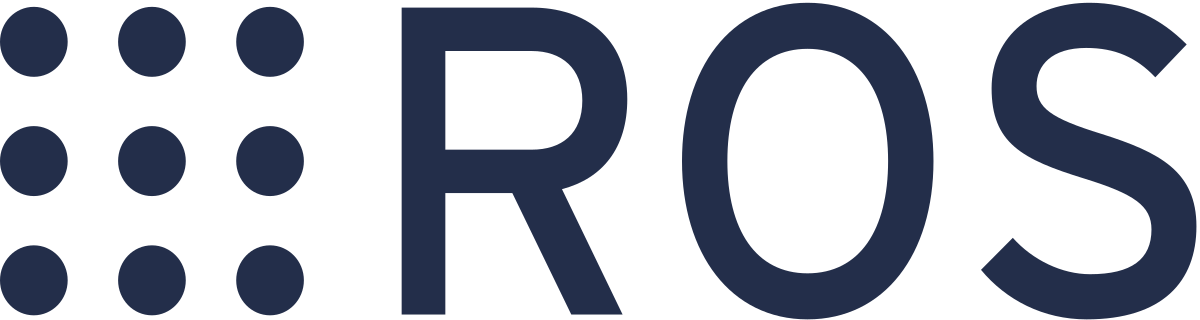
\includegraphics[scale=0.2]{ROSLOGO.png}
    \caption[ROS logo]{ROS logo}
\end{figure}

The Robot Operating System (\acs{ros}) is a set of software libraries and tools that help you build robot applications.
\acs{ros} enables the user to simplify the creation of robust robot applications. Using nodes, \acs{ros} provides an easy method of 
communication between a robot and the user or, in case of multiple robots, between robots themselves.A \acs{ros} node is a process 
that performs computation, it is an executable program \cite{ros:node}. All the nodes are 
connected to ROScore, a collection of \acs{ros} nodes, differentiated by name. Each node can contain multiple topics,with each topic 
assigned a topic name. A topic is a bus over which nodes exchange messages \cite{ros:topic}.
Using this topic name a user can create subscribers (to access information from this topic) and publishers (to add new data to the topic). 
Information can be shared between nodes using these subscribers and publishers from different nodes \cite{ros:about}.

\begin{figure}[ht]
    \centering
    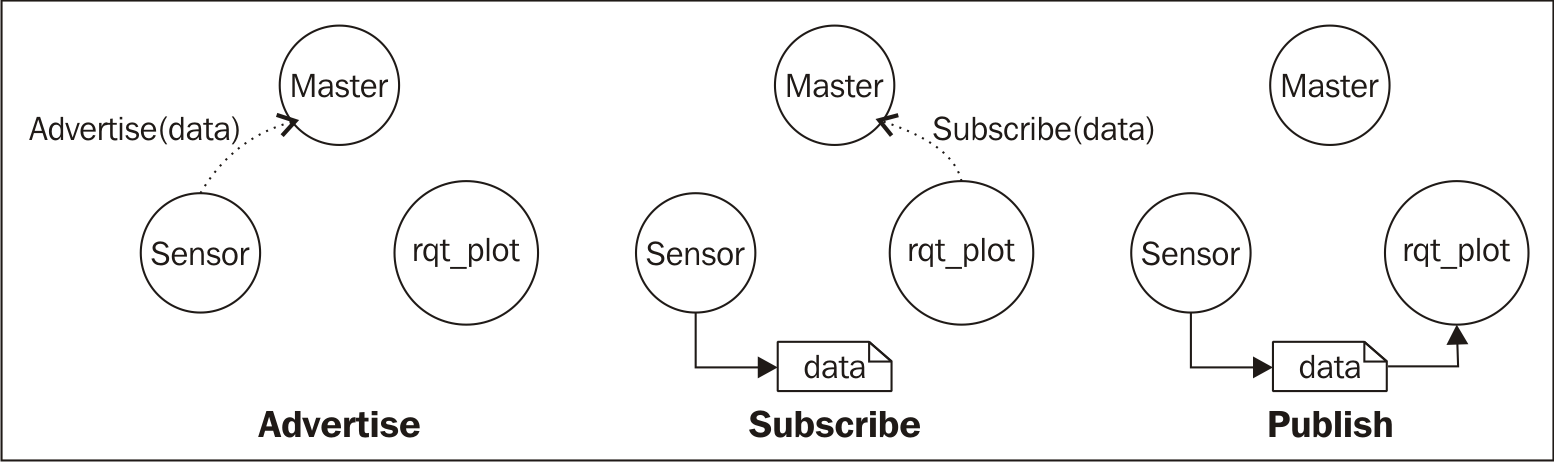
\includegraphics[width=1.0\textwidth]{roscore.png}
    \caption[ROS core]{ROS core}
\end{figure}
